\documentclass[conference]{IEEEtran}

% Packages
\usepackage{cite}
\usepackage{amsmath,amssymb,amsfonts}
\usepackage{algorithmic}
\usepackage{algorithm}
\usepackage{graphicx}
\usepackage[T1]{fontenc}
\usepackage{textcomp}
\usepackage{xcolor}
\usepackage{booktabs}
\usepackage{multirow}
\usepackage{hyperref}

% Math operators
\DeclareMathOperator{\KL}{KL}
\DeclareMathOperator{\Var}{Var}
\DeclareMathOperator{\clip}{clip}

\begin{document}

\title{Playing Balatro with LLM-Guided\\Deep Reinforcement Learning}

% Double-blind: remove author info for submission
\author{
\IEEEauthorblockN{Anonymous}
}

\maketitle

\begin{abstract}
Roguelike deckbuilding games pose unique challenges for reinforcement learning: combinatorial action spaces, long planning horizons, and sparse rewards make pure RL difficult to converge, while the strategic knowledge needed for effective play is well-documented in human-authored game guides.
We present an LLM-guided RL framework for a simplified version of Balatro, a roguelike deckbuilding poker game, that leverages existing game guides through a retrieval-augmented LLM to assist RL agents in knowledge-intensive decisions where exploration alone is insufficient.
Our approach demonstrates the potential of combining LLMs with RL to directly exploit human game knowledge, offering a practical path for training game AI in domains characterized by combinatorial complexity and sparse feedback.
\end{abstract}

\begin{IEEEkeywords}
reinforcement learning, LLM action prior, hesitation gate, card games, roguelike deckbuilder, Balatro, action masking
\end{IEEEkeywords}

% ================================================================
\section{Introduction}
% ================================================================

Reinforcement learning has achieved superhuman performance in games ranging from Atari~\cite{mnih2015human} to StarCraft~II~\cite{vinyals2019grandmaster}, yet roguelike deckbuilding games remain largely unexplored.
These games combine stochastic card draws, combinatorial action spaces, and---crucially---\textit{knowledge-intensive decisions} that depend on understanding complex interactions among hundreds of game elements.
While prior card game research has focused on competitive settings such as poker~\cite{brown2019superhuman} and Hanabi~\cite{bard2020hanabi}, single-player deckbuilders pose a distinct challenge: the strategic knowledge needed (e.g., which modifier cards synergize) is abundantly documented in community guides but prohibitively expensive to discover through exploration alone.

We study \textbf{Balatro}, a roguelike deckbuilding poker game whose different phases demand different reasoning capabilities (Fig.~\ref{fig:gameplay}).
The hand-play phase---selecting which cards to play from an 8-card hand---is a combinatorial optimization problem amenable to standard RL.
The joker selection phase---choosing which modifier cards to equip---requires strategic game knowledge about effect synergies that pure RL struggles to acquire.

This asymmetry motivates our core idea: \textit{use LLMs to inject human game knowledge exactly where RL falls short}.
We treat a retrieval-augmented LLM~\cite{lewis2020retrieval} as a Bayesian action prior~\cite{yan2024efficient} and incorporate it into a PPO agent via variational inference.
To avoid unnecessary LLM overhead, we introduce a \textit{hesitation gate} that activates the prior only when the policy's softmax output exhibits low confidence---effectively implementing the principle ``ask for help when uncertain.''

Our contributions are:
\begin{itemize}
    \item A \textbf{multi-phase RL framework} for Balatro with phase-specific agents for hand-play and joker selection.
    \item A comparison of \textbf{DDQN and PPO} with bitmask action encoding and action masking on the combinatorial hand-play phase.
    \item A \textbf{hesitation-gated LLM prior} that selectively incorporates game strategy knowledge via RAG, reducing LLM queries as the policy gains confidence.
    \item A pure-Python game engine recreating core Balatro mechanics for fast, large-scale RL training.
\end{itemize}

% ================================================================
\section{Balatro: Game Overview}
\label{sec:game}
% ================================================================

In Balatro, the player begins each run with a standard 52-card deck and scores chips by playing poker hands to defeat escalating challenges.
A run progresses through 8 \textit{Antes}, each containing 3 \textit{Blinds} (Small, Big, and Boss) with progressively higher chip thresholds.

\begin{figure}[t]
\centering
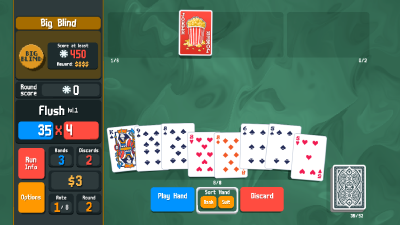
\includegraphics[width=\columnwidth]{figures/Balatro_big_blind.png}
\caption{The hand-play phase in Balatro. The player is dealt 8 cards and must select cards to play as a poker hand or discard. The left panel shows the current blind target, equipped Joker, detected hand type with base scoring values, remaining hands/discards, and current funds.}
\label{fig:gameplay}
\end{figure}

\subsection{Core Game Phases}

\textbf{Hand Play.}
The player is dealt 8 cards from their deck with limited \textit{hands} (typically 4) and \textit{discards} (3) per blind.
Each turn, the player selects 1--5 cards to either play as a poker hand (consuming a hand) or discard and redraw replacements (consuming a discard).
The strategic tension lies in deciding whether to play an available hand immediately or invest discards to improve hand quality.

\textbf{Scoring.}
The score for a played hand is computed as:
\begin{equation}
\small
\mathrm{Score} = \underbrace{(B_c\!+\!C_c\!+\!\Delta_c)}_{\text{Chips}} \times \underbrace{(B_m\!+\!\Delta_m) \times {\textstyle\prod_j} X_m^{(j)}}_{\text{Multiplier}}
\label{eq:score}
\end{equation}
where $B_c, B_m$ are base chips and multiplier from the poker hand type (Table~\ref{tab:handtypes}), $C_c$ is the sum of chip values of scoring cards, and $\Delta_c, \Delta_m, X_m^{(j)}$ are modifiers applied by the $j$-th Joker.
Critically, Jokers are evaluated \textit{left to right}, with multiplicative Jokers ($X_m$) applied immediately to the running multiplier---making Joker \textit{ordering} a non-trivial strategic consideration.

\textbf{Shop Phase.}
After defeating each blind, the player enters a shop where they can spend earned dollars to purchase Jokers, consumables including Tarot cards (22 types), Planet cards (12 types), and Spectral cards (18 types), as well as booster packs and Vouchers (32 types).

\textbf{Blind Selection.}
Before each blind, the player may choose to skip the Small or Big blind for a tag bonus, or face a Boss Blind with a special debuff effect (e.g., all Hearts debuffed, face-down cards, reduced hand size).
The game features 30 distinct blind types.

\begin{table}[t]
\centering
\caption{Poker hand types with base scoring values (Level 1). Planet cards can level up each hand type, permanently increasing its base values.}
\label{tab:handtypes}
\begin{tabular}{lcc}
\toprule
\textbf{Hand Type} & \textbf{Base Chips} & \textbf{Base Mult} \\
\midrule
High Card & 5 & 1 \\
Pair & 10 & 2 \\
Two Pair & 20 & 2 \\
Three of a Kind & 30 & 3 \\
Straight & 30 & 4 \\
Flush & 35 & 4 \\
Full House & 40 & 4 \\
Four of a Kind & 60 & 7 \\
Straight Flush & 100 & 8 \\
Five of a Kind & 120 & 12 \\
\bottomrule
\end{tabular}
\end{table}

\begin{figure}[t]
\centering
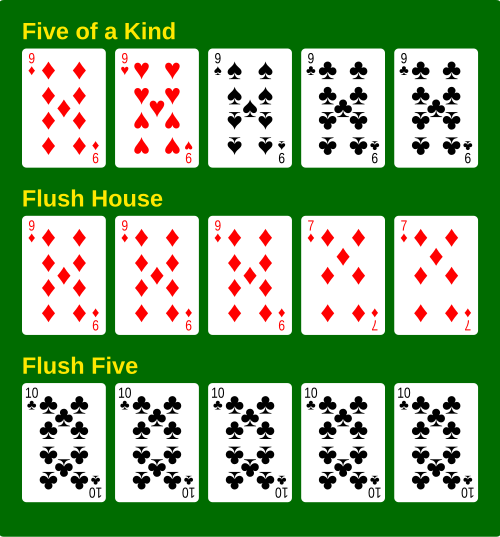
\includegraphics[width=0.7\columnwidth]{figures/Balatro-Special-Poker-Hands.svg.png}
\caption{Balatro introduces special poker hands beyond the standard ranking. \textit{Five of a Kind}: five cards of the same rank. \textit{Flush House}: a Full House where all cards share a suit. \textit{Flush Five}: five identical-rank cards of one suit. These hands yield significantly higher base scores.}
\label{fig:special_hands}
\end{figure}

\subsection{Jokers: The Key Strategic Element}
\label{sec:game:jokers}

The game features 150 unique Joker cards---persistent modifiers that alter scoring in qualitatively different ways.
The player may hold up to 5 Jokers at a time, and can buy, sell, or replace them at the shop between rounds.
Critically, Jokers are evaluated \textit{left to right} during scoring (Eq.~\ref{eq:score}), so their \textit{positional order} directly affects the result: placing a multiplicative Joker after an additive one yields a different score than the reverse.
This means the joker management problem involves not only \textit{which} Jokers to hold but also \textit{in what order} to arrange them---creating a combinatorial explosion.
With 150 Joker types, choosing up to 5 from the available pool yields $\sum_{k=0}^{5}\binom{150}{k} > 5.9 \times 10^8$ subsets, each with up to $5! = 120$ orderings.

Our engine implements 30 representative Jokers spanning several archetypes:
\textit{flat bonus} (e.g., $+4$ Mult),
\textit{conditional} (e.g., $+8$ Mult if the hand contains a Pair),
\textit{suit-based} (e.g., $+3$ Mult per Diamond scored),
\textit{multiplicative} (e.g., $\times 3$ Mult if all held cards are Spades/Clubs), and
\textit{scaling} (e.g., $+15$ Chips per Straight played, cumulative across rounds).
Identifying synergies among Jokers and their optimal ordering---the central strategic challenge---requires knowledge that is well-documented in community guides but expensive to discover through trial and error.

\subsection{Challenges for RL}

Balatro presents five distinguishing challenges that motivate our design choices:
(1) \textbf{Combinatorial action space}: selecting $k$ from 8 cards yields $\sum_{k=1}^{5}\binom{8}{k} = 218$ subsets, doubled for play/discard---addressed by bitmask encoding with action masking;
(2) \textbf{Nonlinear reward}: the multiplicative scoring formula means small changes in card selection can produce order-of-magnitude score differences;
(3) \textbf{Multi-phase planning}: hand-play and joker selection require different agent architectures;
(4) \textbf{Long horizon}: 9 rounds with escalating chip requirements and sparse terminal reward;
(5) \textbf{Knowledge-intensive decisions}: optimal joker selection \textit{and ordering} depends on complex interactions among 150 joker types---motivating our LLM-guided approach.

\subsection{Our Simplified Game Model}

The full Balatro game includes shop management, blind selection, consumable usage, and multi-ante progression.
To focus on the core RL challenges, we construct a simplified two-phase game model:
\begin{itemize}
    \item \textbf{Joker Selection Phase}: At the start of each run, 5 Jokers are randomly sampled from the full pool of 30 implemented types and offered to the agent, who selects which ones to equip (up to 5 slots).
    \item \textbf{Hand-Play Phase}: The agent plays 9 consecutive rounds, each consisting of a deal of 8 cards followed by a sequence of play/discard decisions with limited hands and discards. The equipped Jokers affect scoring throughout all rounds.
\end{itemize}
The game ends automatically after the 9th round.
Crucially, this simplification retains the two signature challenges of roguelike deck-builders that make them difficult for RL:
\begin{enumerate}
    \item \textbf{Combinatorial explosion in Joker selection.} Even with 30 implemented types and 5 slots, the joint space of subsets and orderings remains vast (Section~\ref{sec:game:jokers}), preserving the strategic depth of the original game.
    \item \textbf{Long-horizon, sparse rewards.} A single Joker choice propagates through all 9 subsequent rounds, yet the agent receives only a cumulative score at the end of the run. This delayed credit-assignment problem is characteristic of roguelikes, where early decisions compound over extended play horizons.
\end{enumerate}
By stripping away shop economics and blind selection, we isolate these core difficulties and create a tractable testbed for investigating how LLM priors can accelerate RL in combinatorially rich, sparse-reward settings.

% ================================================================
\section{Environment Design}
\label{sec:env}
% ================================================================

Rather than hooking into the original Lua-based game, we build a \textit{custom simplified environment} in pure Python that reproduces core Balatro mechanics.
The environment is not a faithful replica of the full game: it implements the simplified two-phase model from Section~\ref{sec:game} (joker selection followed by 9 rounds of hand play), omitting shop economics, blind selection, consumables, and multi-ante progression.
This design choice prioritizes fast, deterministic simulation for large-scale RL training over completeness.

\subsection{Hand-Play Environment}
\label{sec:handplay_env}

The hand-play phase is formulated as an episodic MDP $(\mathcal{S}, \mathcal{A}, P, R, \gamma)$.

\textbf{State Space.}
A 57-dimensional vector encoding 8 card slots ($8 \times 6$: suit, rank, chip value, debuff, face-card, existence, all normalized) and game state (9 dims: hands/discards remaining, hand/deck size, score).

\textbf{Action Space.}
Bitmask encoding (Discrete 510): actions 0--254 encode \textbf{play} with card mask $m = \text{action}+1 \in \{1,...,255\}$ (bit $i$ selects card $i$), and actions 255--509 encode \textbf{discard} with the same mask.

\textbf{Action Masking.}
A boolean mask enforces card existence, at-most-5 selection, and hand/discard availability.

\textbf{Reward.}
Sparse terminal reward: $R_t = 0$ for non-terminal steps, $R_T = \text{total\_score}$ (cumulative score over all 9 rounds), with $\gamma = 1$.

\subsection{Joker Selection Environment}

A separate Gymnasium environment handles joker selection. At the start of each episode, the environment samples 5 Jokers from the 30 implemented types. The agent observes their attributes (89-dimensional vector encoding joker effects and game context) and selects which to equip (up to 5 slots). The chosen jokers persist throughout all 9 rounds, affecting every scoring calculation.

% ================================================================
\section{Method}
\label{sec:method}
% ================================================================

Our framework assigns a specialized agent to each game phase: Section~\ref{sec:handplay_agents} compares DDQN and PPO for hand-play, and Section~\ref{sec:llm_prior} describes the PPO agent with hesitation-gated LLM prior for joker selection.

\subsection{Hand-Play Agents}
\label{sec:handplay_agents}

We evaluate two RL approaches for hand-play, both using the bitmask action encoding and action masking from Section~\ref{sec:handplay_env}.

\textbf{DDQN.} Double DQN~\cite{vanhasselt2016deep} with action masking: invalid actions receive $Q = -\infty$ during both selection and $\epsilon$-greedy exploration. Since $\gamma=1$ with sparse terminal reward, we use Monte Carlo returns---every transition target is simply $y_t = R_T$---eliminating bootstrapping error.

\textbf{PPO with Action Masking.} PPO~\cite{schulman2017proximal} with a masked categorical distribution: invalid logits are set to $-\infty$ before softmax, ensuring zero probability on illegal moves~\cite{huang2022closer}. Both agents use identical network capacity to enable fair comparison of value-based versus policy-based methods.

\subsection{Joker Agent: PPO with Hesitation-Gated LLM Prior}
\label{sec:llm_prior}

Joker selection requires strategic knowledge about effect synergies that is abundant in game guides but expensive to learn from scratch. We incorporate this knowledge by treating an LLM as a Bayesian action prior within a PPO framework~\cite{yan2024efficient}, gated by a novel confidence-based mechanism.

\subsubsection{LLM as Action Prior via RAG}

We construct an action prior $p_{\mathrm{LLM}}(a|s)$ using a language model augmented with Retrieval-Augmented Generation (RAG)~\cite{lewis2020retrieval}. Given state $s$ (a text description of available jokers, deck composition, and current ante), the system:
\begin{enumerate}
    \item Retrieves relevant passages from a curated knowledge base of Balatro strategy guides.
    \item Prompts the LLM with the retrieved context and state, asking it to select the best action.
    \item Repeats the query $N$ times independently. The empirical action frequencies form the prior: $p_{\mathrm{LLM}}(a|s) = n_a / N$, where $n_a$ is the number of times action $a$ was chosen across $N$ queries.
\end{enumerate}

\subsubsection{Bayesian Framework: Variational Inference with LLM Prior}

Following~\cite{yan2024efficient, levine2018reinforcement}, we frame RL as Bayesian inference. An optimality variable $\mathcal{O}$ indicates trajectory quality with likelihood $p(\mathcal{O}{=}1 \mid \tau) \propto \exp\!\bigl(\sum_t \gamma^t r_t / \alpha\bigr)$. The trajectory prior factorizes as:
\begin{equation}
\small
p(\tau) = p(s_0)\!\prod_{t=0}^{T} p_{\mathrm{LLM}}(a_t | s_t)\, P(s_{t+1} | s_t, a_t)
\end{equation}

Using variational inference with $q(\tau) = p(s_0)\prod_t \pi_\theta(a_t \mid s_t)\,P(s_{t+1} \mid s_t, a_t)$ as the variational distribution, maximizing the ELBO yields:
\begin{equation}
\small
\max_\theta\; \mathbb{E}_{\pi_\theta}\!\Bigl[\sum_{t} \gamma^t r_t - \alpha \, \KL\bigl[\pi_\theta(\cdot|s_t) \big\| p_{\mathrm{LLM}}(\cdot|s_t)\bigr]\Bigr]
\label{eq:vi_objective}
\end{equation}

This objective balances reward maximization with proximity to the LLM prior, regularizing the policy toward expert-like behavior while permitting adaptation through online interaction.

\subsubsection{Hesitation Gate}

Invoking the LLM at every step is costly, and when the policy is already confident the prior may add noise rather than useful signal. We propose a \textit{hesitation gate} that activates the LLM prior only when the policy exhibits uncertainty.

\textbf{Motivation.}
The key observation is that a policy's softmax output reveals \textit{how much it knows}.
When the variance across action probabilities is low, the distribution is nearly uniform---the agent assigns similar probability to many actions and has no strong preference.
This ``hesitation'' signals that the agent lacks sufficient knowledge to distinguish good actions from bad ones, which is precisely the situation where external guidance from the LLM is most valuable.
Conversely, when the variance is high---indicating a peaked distribution with a clear preferred action---the agent has already learned a confident strategy, and injecting the LLM prior would only add noise or computational overhead.
The hesitation gate formalizes this intuition: \textit{consult the LLM when the policy hesitates, trust the policy when it is confident}.

\textbf{Confidence measure.} Given the PPO policy's softmax output $\pi_\theta(\cdot \mid s) = [p_1, \ldots, p_n]$ where $n = |\mathcal{A}|$, we compute the normalized variance:
\begin{equation}
\small
h(s) = \frac{\Var\bigl(\pi_\theta(\cdot|s)\bigr)}{\sigma^2_{\max}}, \quad
\sigma^2_{\max} = \frac{n-1}{n^2}
\label{eq:hesitation}
\end{equation}
where $\Var(\pi) = \frac{1}{n}\sum_{i=1}^{n}(p_i - \frac{1}{n})^2$ and $\sigma^2_{\max}$ is the variance of a one-hot distribution. The measure $h(s) \in [0, 1]$: $h = 0$ for a uniform distribution (maximum uncertainty) and $h = 1$ when all mass is on a single action (maximum confidence).

\textbf{Gate activation.} The gate function is:
\begin{equation}
\small
g(s) =
\begin{cases}
1 & h(s) < \tau \;\;\text{(uncertain --- use LLM)} \\[3pt]
0 & h(s) \geq \tau \;\;\text{(confident --- skip LLM)}
\end{cases}
\label{eq:gate}
\end{equation}
where $\tau \in (0, 1)$ is a threshold hyperparameter.

\textbf{Combined objective.} Incorporating the hesitation gate into the PPO framework, the policy is optimized by:
\begin{equation}
\small
\begin{aligned}
L(\theta) = \mathbb{E}_{\pi_{\theta_{\mathrm{old}}}}\Bigl[
  & \clip\!\bigl(r_t(\theta)\,\hat{A}_t,\; 1\!\pm\!\epsilon\bigr) \\
  &+ \beta\, H\!\bigl(\pi_\theta(\cdot|s_t)\bigr) \\
  &- g(s_t)\,\alpha\, \KL\bigl[\pi_\theta(\cdot|s_t) \big\| p_{\mathrm{LLM}}(\cdot|s_t)\bigr] \Bigr]
\end{aligned}
\label{eq:ppo_prior}
\end{equation}
where $r_t(\theta) = \pi_\theta(a_t|s_t) / \pi_{\theta_{\mathrm{old}}}(a_t|s_t)$ is the probability ratio, $\hat{A}_t$ is the estimated advantage, $\beta$ controls entropy regularization, and $\alpha$ weights the LLM prior influence. When the gate is off ($g\!=\!0$), this reduces to standard PPO; when on ($g\!=\!1$), the KL term pulls the policy toward the LLM's recommendations.

\textbf{Intuition.} A near-uniform softmax signals that the policy cannot distinguish between actions---precisely when external knowledge is most valuable. As training progresses and confidence grows, the gate activates less frequently, naturally transitioning from LLM-guided to autonomous behavior.

\begin{algorithm}[t]
\caption{Hesitation-Gated PPO with LLM Prior}
\label{alg:hg_ppo}
\begin{algorithmic}[1]
\STATE Initialize policy $\pi_\theta$, value function $V_\phi$
\STATE Load RAG knowledge base from game guides
\FOR{each iteration}
    \STATE Collect trajectories using $\pi_\theta$
    \FOR{each state $s_t$ in batch}
        \STATE Compute $h(s_t)$ via Eq.~\ref{eq:hesitation}
        \IF{$h(s_t) < \tau$}
            \STATE Query LLM with RAG: $p_{\mathrm{LLM}}(\cdot \mid s_t)$
            \STATE Compute $\KL\bigl[\pi_\theta(\cdot \mid s_t) \,\big\|\, p_{\mathrm{LLM}}(\cdot \mid s_t)\bigr]$
        \ELSE
            \STATE Set KL term $= 0$
        \ENDIF
    \ENDFOR
    \STATE Update $\theta$ by maximizing $L(\theta)$ (Eq.~\ref{eq:ppo_prior})
    \STATE Update $\phi$ by minimizing value loss
\ENDFOR
\end{algorithmic}
\end{algorithm}

% ================================================================
\section{Experiments}
\label{sec:results}
% ================================================================

Our experiments address three questions: (1)~How do DDQN and PPO compare on combinatorial hand-play? (2)~Does the hesitation-gated LLM prior improve joker selection over pure PPO? (3)~Does the full two-phase pipeline outperform single-phase baselines?

\subsection{Experimental Setup}

All experiments use our pure-Python engine on consumer hardware. Both DDQN and PPO agents use identical network capacity, sparse terminal reward with $\gamma=1$, and are trained for 1M episodes.

\subsection{Experiment 1: Hand-Play Phase (DDQN vs. PPO)}

DDQN and PPO with action masking are compared against a random baseline (uniform over valid actions).
Both agents use sparse terminal reward with $\gamma=1$ and identical network capacity.
Metrics: mean terminal score, maximum score, and sample efficiency (episodes to reach 90\% of final performance).
A reward ablation compares sparse terminal reward against shaped per-step reward.

\subsection{Experiment 2: Joker Selection with LLM Prior}

The hesitation-gated LLM prior is evaluated on joker selection by comparing four conditions:
\begin{itemize}
    \item \textbf{Random}: Uniform random joker selection.
    \item \textbf{PPO}: Standard PPO without LLM guidance.
    \item \textbf{PPO + LLM Prior}: PPO with constant KL regularization toward the LLM prior (Eq.~\ref{eq:vi_objective}, no gate).
    \item \textbf{PPO + Hesitation Gate}: Our full method (Eq.~\ref{eq:ppo_prior}), with LLM prior activated only when policy confidence is low.
\end{itemize}
Performance is measured by total score over 9 rounds with a fixed trained hand-play agent.
A central goal of this experiment is to quantify the \textit{efficiency--performance trade-off} of the hesitation gate: we report
(1)~\textbf{LLM query reduction}---the percentage of LLM calls saved by the gated method compared to the always-on prior (PPO + LLM Prior), and
(2)~\textbf{performance retention}---the fraction of the always-on prior's score achieved by the gated variant despite fewer queries.
We additionally track gate activation rate over training to verify the expected transition from LLM-guided to autonomous behavior: early in training, when the policy is near-uniform and the gate fires frequently, and late in training, when the policy has converged and the gate activates rarely.

\subsection{Experiment 3: Hesitation Gate Ablation}

We study sensitivity to three hyperparameters:
\begin{itemize}
    \item \textbf{Threshold $\tau$}: We sweep $\tau \in \{0.1, 0.2, 0.3, 0.5, 0.7\}$ to characterize the trade-off between LLM query frequency and performance.
    \item \textbf{KL weight $\alpha$}: We test $\alpha \in \{0.01, 0.1, 0.5, 1.0\}$ to measure the influence strength of the LLM prior.
    \item \textbf{Confidence measure}: We compare our normalized-variance measure against entropy-based and max-probability-based alternatives.
\end{itemize}

\subsection{Experiment 4: End-to-End Evaluation}

The full two-phase pipeline is evaluated end-to-end: a trained joker agent (with or without LLM prior) feeds its selections into a trained hand-play agent for 9 rounds.
Comparison against single-phase baselines (random jokers, random play) quantifies the synergy between the two trained components.

% ================================================================
\section{Related Work}
\label{sec:related}
% ================================================================

\textbf{RL for games.}
Deep RL has progressed from Atari~\cite{mnih2015human} through strategy games like StarCraft~II~\cite{vinyals2019grandmaster} and Dota~2~\cite{berner2019dota} to open-ended environments such as NetHack~\cite{kuttler2020nethack}, Minecraft~\cite{guss2019minerl}, and Pok\'emon Red~\cite{pleines2025pokemon}.
Card games introduce stochasticity and imperfect information: Pluribus~\cite{brown2019superhuman} achieved superhuman poker play, and Hanabi~\cite{bard2020hanabi} tests cooperative reasoning under partial observability.
Hearthstone has been approached with MCTS~\cite{santos2017monte} and Slay the Spire with search methods~\cite{saavedraSTS2024}.
Balatro differs from these as a \textit{single-player} roguelike deckbuilder where the primary challenge is combinatorial optimization over card subsets and modifier selection---no opponent modeling is required, but strategic knowledge about card synergies is essential.

\textbf{Incorporating external knowledge into RL.}
One line of work uses LLMs as reward shapers or value guides~\cite{zhang2024llmguide}; another treats LLM outputs as action priors within a Bayesian framework~\cite{yan2024efficient, levine2018reinforcement}. We follow the latter approach but introduce two novelties: (1)~a hesitation gate that conditions LLM engagement on policy confidence, reducing unnecessary queries, and (2)~application to a card game domain where RAG over human-authored strategy guides provides the prior knowledge.
Action masking~\cite{huang2022closer} is orthogonal and critical for sample efficiency in our large discrete action space; we apply it in both DDQN and PPO agents.

% ================================================================
\section{Discussion and Limitations}
\label{sec:discussion}
% ================================================================

\textbf{Hesitation gate design.} Our normalized-variance gate is simple and interpretable but not the only option---entropy or max-probability measures are natural alternatives. The threshold $\tau$ trades off query cost against guidance benefit; adaptive thresholds that evolve during training are a promising direction.

\textbf{LLM overhead.} Each RAG query introduces latency. The hesitation gate reduces query frequency as training progresses, and policy distillation could further amortize LLM costs for real-time play.

\textbf{Simplified game scope.} Our environment implements 30 of 150+ Joker types and omits shop management, blind selection, and consumables. This suffices for validating the methodology, but a complete implementation is needed for human-level comparison.

\textbf{Ongoing evaluation.} The experimental framework is designed; full results are pending. We present planned experiments to enable reproducibility and invite community evaluation.

% ================================================================
\section{Conclusion}
\label{sec:conclusion}
% ================================================================

We presented an RL framework for Balatro that addresses different game phases with appropriate methods: DDQN and PPO are compared on the combinatorial hand-play phase, while a hesitation-gated LLM prior injects human game knowledge into joker selection exactly when the policy is uncertain.
The hesitation gate provides a principled, confidence-aware mechanism for engaging LLM guidance that naturally reduces query frequency as training progresses.

Future work includes: (1)~full experimental evaluation of the LLM-guided joker agent; (2)~expanding to all 150+ Joker types with shop and blind selection phases; (3)~end-to-end multi-phase training; and (4)~comparison against human experts.

Our framework is publicly available to support research on RL for combinatorial card games.\footnote{Repository URL omitted for double-blind review.}

% ================================================================
\bibliographystyle{IEEEtran}
\bibliography{references}

\end{document}
